\documentclass[11pt]{article}
\usepackage[utf8]{inputenc}
\usepackage[margin=0.9in]{geometry}
\geometry{a4paper}
\linespread{1} %全局行距

\usepackage{amsmath}
\usepackage{amssymb}
\usepackage{amsthm}
\usepackage{amsfonts}
\usepackage{comment}
\usepackage{booktabs}
\usepackage{array}
\usepackage{paralist}
\usepackage{verbatim}
\usepackage{fancyvrb}
\usepackage{multirow}
\usepackage{rotating}
\usepackage{fancyhdr}
\pagestyle{fancy} %全文使用的pagestyle
\renewcommand{\headrulewidth}{0pt}
\lhead{}\chead{}\rhead{}
\lfoot{}\cfoot{\thepage}\rfoot{}
\usepackage{sectsty}
\allsectionsfont{\sffamily\mdseries\upshape}
\usepackage{algorithm}
\usepackage{algpseudocode}
\usepackage[section]{placeins} %图片


\usepackage{natbib}
\bibliographystyle{abbrvnat}
\usepackage{filecontents} %允许把bib写在tex里


\usepackage{CJKutf8}
\usepackage{cprotect}
\usepackage{booktabs}
\usepackage[dvipsnames]{xcolor} %代码高亮+ref额外颜色
\usepackage[toc,title,titletoc]{appendix} %附录

\usepackage{graphicx}
\usepackage{float}%设置图片浮动位置
\usepackage[labelformat=simple]{subcaption} %更先进的子图包
\renewcommand\thesubfigure{(\alph{subfigure})}

\usepackage{hyperref}
\hypersetup{
	colorlinks=true,%会取消边框
	linkcolor=blue,
	filecolor=cyan,
	urlcolor=magenta,
	anchorcolor=red,
	citecolor= Green
}
%%% 比较丑的Python

\setlength{\parindent}{0em} %段首不缩进
\setlength{\parskip}{1ex} %段间空一行

\definecolor{codegrey}{HTML}{F8F8F8}
\usepackage{listings} %插入代码

\lstdefinestyle{lfonts}{
  basicstyle   = \footnotesize\ttfamily,
  stringstyle  = \color{purple},
  keywordstyle = \color{blue!60!black}\bfseries,
  commentstyle = \color{olive},
}
\lstdefinestyle{lnumbers}{
  numbers     = none,
  numberstyle = \tiny,
  numbersep   = 1em,
  firstnumber = 1,
  stepnumber  = 1,
}
\lstdefinestyle{llayout}{
  breaklines       = true,
  tabsize          = 2,
  columns          = fullflexible,
  backgroundcolor = \color{codegrey},
}
\lstdefinestyle{lgeometry}{
  xleftmargin      = 0pt,
  xrightmargin     = 0pt,
  frame            = tb,
  framesep         = \fboxsep,
  framexleftmargin = 0pt,
}
\lstdefinestyle{lgeneral}{
  style = lfonts,
  style = lnumbers,
  style = llayout,
  style = lgeometry,
}
\lstdefinestyle{python}{
    language = {Python},
    style    = lgeneral,
}


\title{MATH  70076 Data Science \\ Assessed Coursework 1\\ Active mines in the U.S.}
\author{CID: 02242799}
\date{5 February 2023}
\begin{document}
\begin{CJK}{UTF8}{gbsn}
\maketitle

The \href{https://www.msha.gov/data-and-reports}{data} on the Mine industry collected by the Department of Labor's Mine Safety and Health Administration  \href{https://www.msha.gov/}{(MSHA)} of the U.S. provides massive information about this industry. The following paragraphs will base on the \href{https://wwwn.cdc.gov/niosh-mining/MMWC#disasters}{active mine dataset} published by MSHA and visualise it accompanied by corresponding analysis.

The following Figure \ref{fig:act1} shows the number of active mines in 5 sectors in the U.S. from 1983 to 2021. The coal and metal sector showed a downward trend throughout the period, while active stone mines increased. The active coal mine has decreased significantly over the last 39 years. It sharply reduced from around 5500 in 1983 to 800 in 2021. The highest number of active mines remains to be Sand \& gravel sector, which fluctuated between 5500 and 7250. The two lowest mine sectors are metal and non-metal. The non-metal mine decreased steadily, falling from 800 to around 350 and remained the lowest, while the mines of non-metal remained steady throughout the period.

\begin{figure}[h]
  \centering
  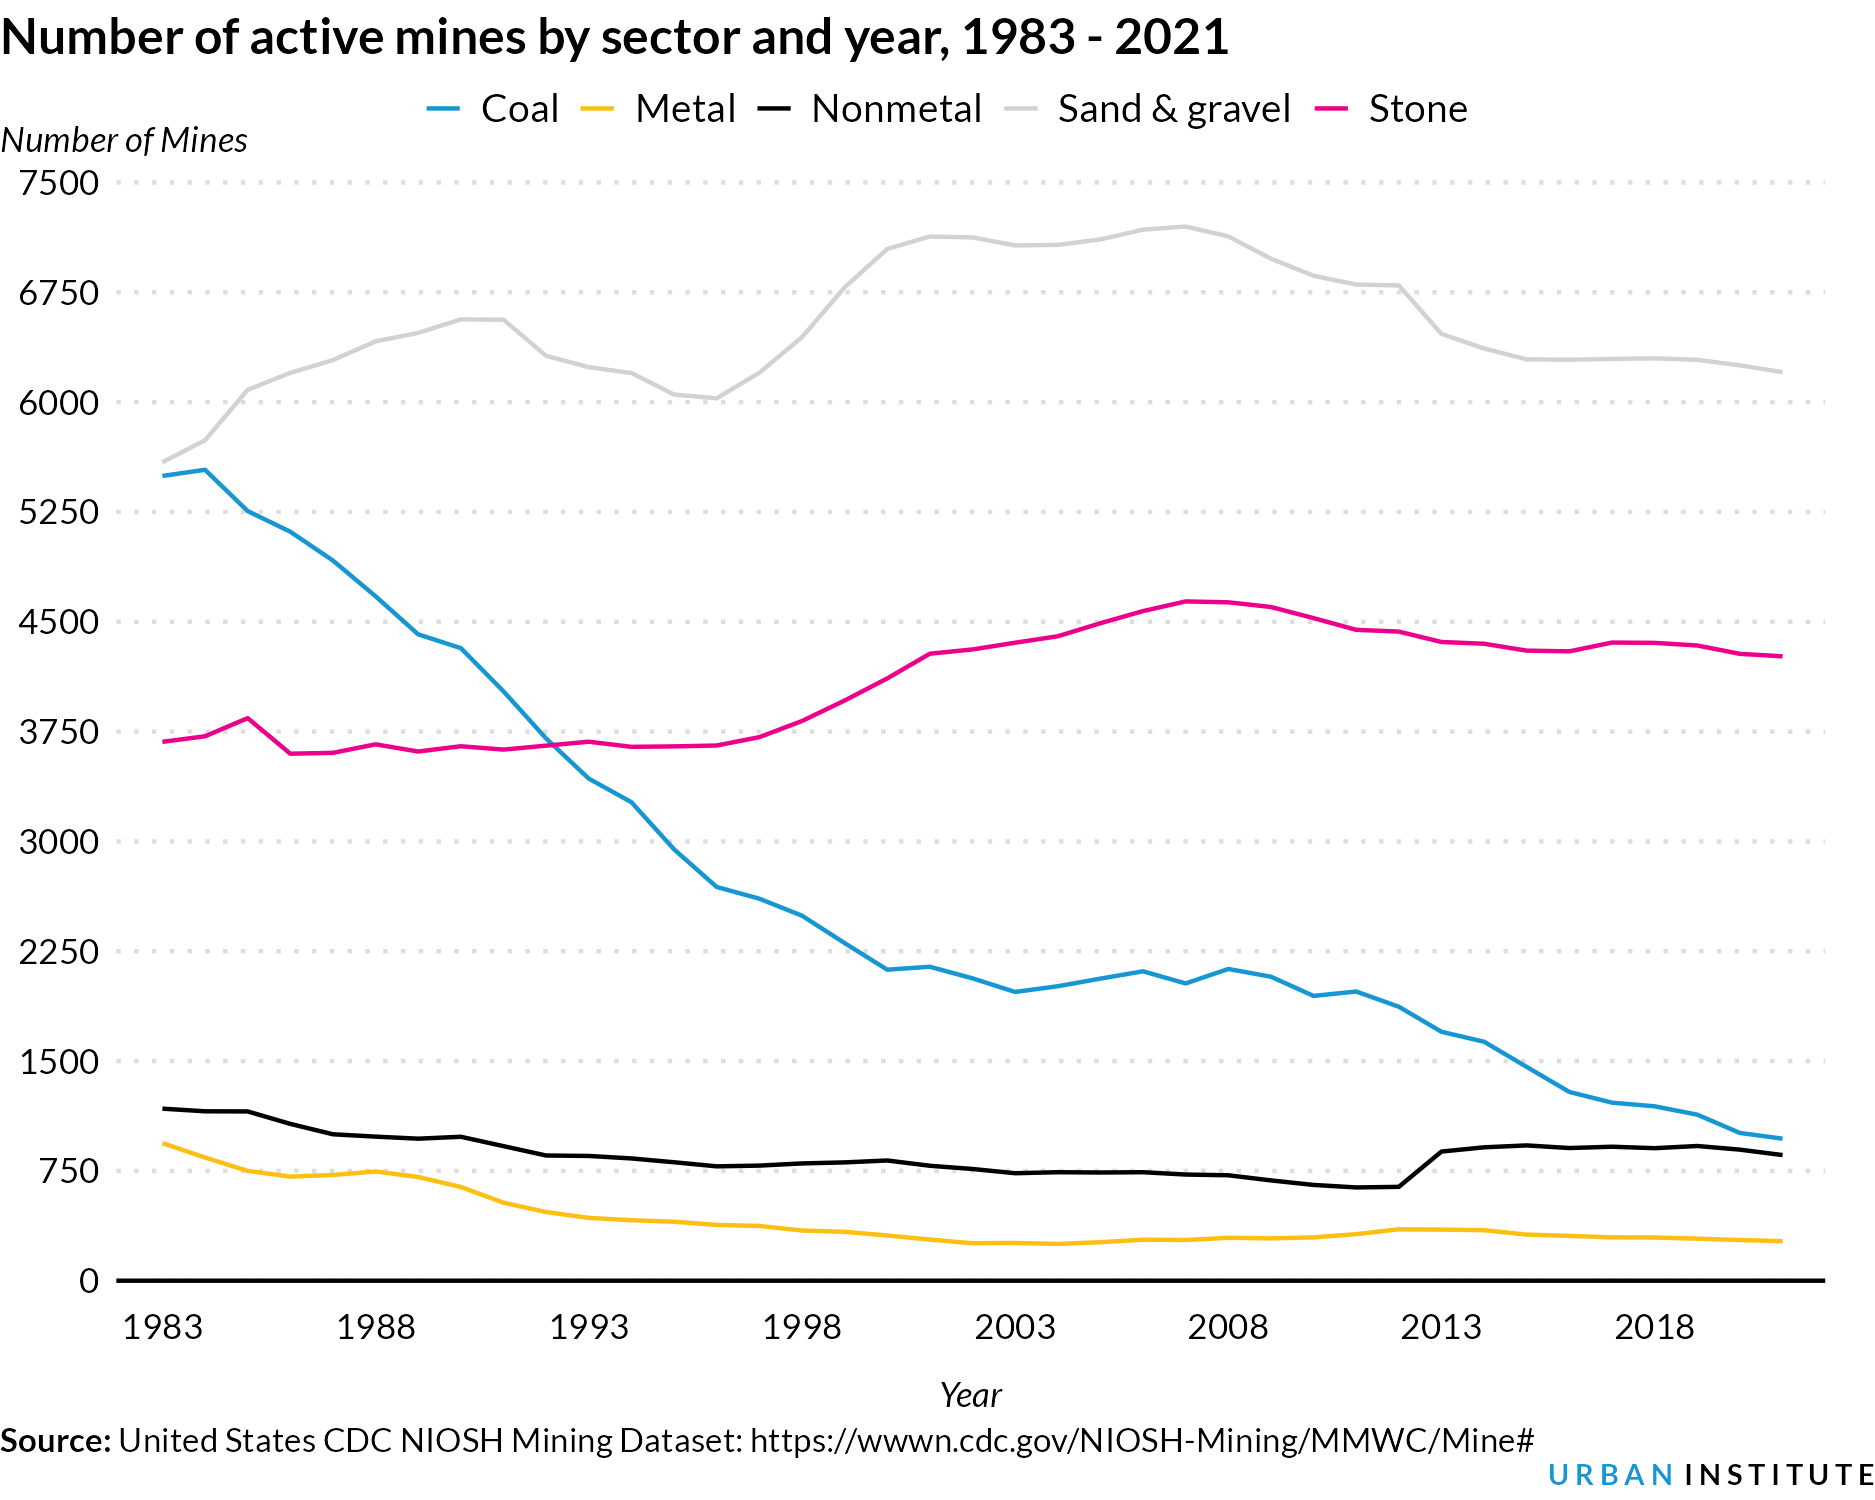
\includegraphics[width=12cm]{../outputs/opt_num_plot.png}
  \caption{Number of active mines by sector and year, 1983 - 2021}
  \label{fig:act1}
\end{figure}

Figure \ref{fig:act2} shown below illustrates the total number of active mines in 50 states in the U.S. between 1983 and 2021. About 10 states have witnessed an increasing trend throughout the period, while nearly 25 states showed a downward tendency. In addition, the remaining 15 states fluctuated across the period. The states that showed an increasing trend are mainly in the middle north and northeast, while Texas is the only one located in the south. By contrast, most central and southern states experienced a declining trend. In 1983, Kentucky (1813), Pennsylvania (1407) and West Virginia (1126) had the most active mines, while 39 years later, Taxes (800), Pennsylvania (704) and Wisconsin (629) had the most. Besides, Delaware and Hawaii remained the states with the least active mine. The mine in Kentucky changed the most, declining from 1813 to 320.

\begin{figure}[h]
  \centering
  \includegraphics[width=\textwidth]{../outputs/opt_state_plot.png}
  \caption{Number of active mines by state and year, 1983 - 2021}
  \label{fig:act2}
\end{figure}





\clearpage



\end{CJK}
\end{document}




